\documentclass[11pt,a4paper]{article}

% Essential Packages
\usepackage[utf8]{inputenc}
\usepackage[margin=1.0in]{geometry}
\usepackage{amsmath,amssymb,amsfonts}
\usepackage{booktabs}
\usepackage{graphicx}
\usepackage[numbers,sort&compress]{natbib}
\usepackage{microtype}
\usepackage{xcolor}
\usepackage{caption}
\usepackage{subcaption}
\usepackage{tabularx}
\usepackage{authblk}
\usepackage{hyperref}

% Hyperref setup with clear academic link colors
\hypersetup{
    colorlinks=true,
    linkcolor=blue!70!black,
    citecolor=blue!70!black,
    urlcolor=blue!80!black
}

% Ensure natbib's \doi command creates a clean clickable blue hyperlink
\makeatletter
\def\doi#1{\href{https://doi.org/#1}{\texttt{doi:#1}}}
\makeatother

\title{\textbf{Rigorous Benchmarking and De-Biasing of Machine Learning Predictors for Antimicrobial Peptides: Resolving Homology Leakage and Negative Sampling Artifacts}}

\author[1]{Ronie Martínez\thanks{Corresponding author: \texttt{ronie.martinez@epn.edu.ec}}}
%\author[1]{Co-investigadores}
\affil[1]{Departamento de Inform{\'a}tica y Ciencias de la Computaci{\'o}n, Escuela Polit{\'e}cnica Nacional, Quito, Ecuador}

%\date{\today}
\date{}

\begin{document}

\maketitle

\begin{abstract}
\textbf{Motivation:} Antimicrobial peptides (AMPs) represent vital therapeutic candidates against the global crisis of antimicrobial resistance (AMR). Although numerous computational tools report near-perfect classification performance ($\text{AUROC} > 0.96$), their real-world experimental translation remains strikingly low. This performance discrepancy is driven by two pervasive flaws: (1) \textit{homology-driven data leakage}, where unconstrained random splitting assigns evolutionary relatives across training and test partitions; and (2) \textit{negative sampling bias}, where random non-AMP background slices transform classification into a trivial discrimination of net charge rather than genuine membrane-disruptive biophysics.\\
\textbf{Methods:} We introduce \textbf{AMP-LeakGuard}, an open-source benchmarking framework that systematically audits and de-biases bioactive peptide classifiers. Using 1,026 manually curated, non-redundant Swiss-Prot AMPs (10--50 amino acids) and 500 reviewed eukaryotic background proteins, we designed two contrasting negative regimes: Scheme A (naive random background slices) and Scheme B (physicochemically matched background slices paired in length and net charge). We evaluated Random Forest and LightGBM models under standard random splitting versus single-linkage homology clustering ($\text{identity} \ge 40\%$) implemented via \texttt{StratifiedGroupKFold}, verified by global dynamic-programming alignment.\\
\textbf{Results:} Our large-scale benchmark ($N = 2,052$ sequences per regime) confirms that naive random cross-validation systematically overestimates performance. Transitioning to a homology-controlled cross-validation regime (verified mean cross-fold global alignment identity of only 16.1\%) yields reproducible degradation across all metrics ($\Delta\text{MCC} = +0.038$ to $+0.053$). More critically, TreeExplainer SHAP reveals that models in Scheme A rely heavily on net charge per residue as an electrostatic shortcut ($\text{mean } |\text{SHAP}| = 0.5475$). When this artifact is neutralized in Scheme B, models are forced to learn genuine biophysical determinants of bacterial lysis: Arginine content (0.8890, reflecting guanidinium bidentate hydrogen bonding), Cysteine content (0.7598, reflecting disulfide cross-linking in defensins), and amphipathic hydrophobic moment (0.7453).\\
\textbf{Conclusions:} Homology-aware partitioning and electrostatic-controlled negative sampling are indispensable prerequisites for establishing reliable predictive pipelines. We establish a four-point guideline aligned with DOME standards to ensure translational viability from computational screening to wet-lab validation.\\
\textbf{Keywords:} Antimicrobial Peptides, Data Leakage, Homology Partitioning, Negative Sampling Bias, Explainable AI, Machine Learning Benchmarking, Membrane Permeabilization.
\end{abstract}

\section{Introduction}

Antimicrobial resistance (AMR) constitutes one of the most formidable public health threats of the 21st century, projected to cause over 10 million deaths annually by 2050 with cumulative economic losses exceeding \$100 trillion \cite{oneill2016tackling}. Conventional small-molecule antibiotics, which largely target stereospecific bacterial enzymes, are increasingly rendered ineffective by point mutations, enzymatic cleavage, and multidrug efflux pump overexpression \cite{blair2015molecular}.

In response, \textbf{antimicrobial peptides (AMPs)} have emerged as promising therapeutic alternatives \cite{mahlapuu2016antimicrobial, lazzaro2020antimicrobial, hancock2006antimicrobial, kumar2018antimicrobial}. Comprising 10 to 50 amino acid residues, canonical AMPs exhibit amphipathic conformations and a net positive charge (typically $+2$ to $+9$ at physiological pH) \cite{zasloff2002antimicrobial}. Their primary mechanism of action relies on biophysical membrane permeabilization: cationic side chains drive electrostatic recruitment to negatively charged bacterial surface lipids (lipopolysaccharide, teichoic acids, phosphatidylglycerol), while hydrophobic patches partition into the fatty acyl core, inducing transmembrane pore formation, membrane curvature, or micellar bilayer disruption \cite{brogden2005antimicrobial, wimley2010describing, matsuzaki2009control, wimley2011antimicrobial}. Because remodeling membrane bilayer chemistry requires complex alterations in lipid synthesis pathways, bacterial resistance against membrane-lytic AMPs evolves at significantly lower frequencies than against conventional antibiotics \cite{spohn2019integrated}.

Over the past decade, high-throughput chemical peptide synthesis has remained resource-intensive, accelerating the development of computational machine learning (ML) and deep learning (DL) predictors based on Random Forests, Support Vector Machines, recurrent and convolutional neural networks, graph attention networks, and pre-trained protein language models \cite{lin2023evolutionary, yan2020deep, notin2023proteingym, veltri2018deep, li2022amplify, santos2020macrel, xu2023iampcn, sharma2021deep, burdukiewicz2020ampgram, capecchi2021machine, yan2021samppfp, ma2022identification}. Published studies routinely report near-perfect discrimination, citing Areas Under the ROC Curve ($\text{AUROC}$) exceeding 0.95 or 0.98 \cite{yan2020deep, veltri2018deep, xu2023iampcn}.

Despite these theoretical successes, \textbf{the translational rate of computationally predicted AMPs in experimental wet-lab assays remains strikingly low} \cite{cardoso2020computer, porto2018silico, torres2019synthetic, capecchi2021machine}. Candidate peptides synthesized based on high predicted probabilities frequently exhibit negligible antimicrobial potency ($\text{MIC} > 128\,\mu\text{g/mL}$) or severe eukaryotic cytotoxicity and hemolysis \cite{cardoso2020computer, torres2019synthetic}. Methodological investigations across computational biology and biomedical artificial intelligence have pinpointed that this discrepancy stems from systemic evaluation pitfalls, shortcut learning, and data leakage \cite{bernett2024guiding, pintor2026antimicrobial, sidorczuk2022benchmarks, geirhos2020shortcut, kapoor2023leakage, whalen2022navigating, roberts2021common, park2012flaw, walsh2021dome}:

\begin{enumerate}
    \item \textbf{Homology-Driven Data Leakage:} Primary databases such as APD3 \cite{wang2016apd3}, DBAASP \cite{pirtskhalava2021dbaasp}, CAMP \cite{waghu2016camp}, DRAMP 3.0 \cite{shi2022dramp}, and dbAMP 2.0 \cite{jhong2022dbamp} are heavily enriched with homologous variants originating from alanine scans, mutagenesis series, or orthologous gene duplications across related amphibian or insect species. When standard random train-test splitting (or standard $k$-fold cross-validation) is applied, variants sharing $>70$--$90\%$ sequence identity inevitably populate both training and evaluation splits \cite{bernett2024guiding, pintor2026antimicrobial}. Under unconstrained random splitting, models simply memorize sequence motifs of overrepresented homologous families rather than learning generalizable biophysical rules, a classic failure mode of biological machine learning \cite{whalen2022navigating, bernett2024guiding, kapoor2023leakage}.
    \item \textbf{Negative Sampling Bias (Electrostatic Shortcut Learning):} Because no centralized repository of confirmed ``non-antimicrobial peptides'' exists, researchers routinely harvest negative samples by carving random subsequences from unannotated UniProt proteins \cite{sidorczuk2022benchmarks}. However, background eukaryotic proteomes predominantly display neutral or acidic isoelectric points \cite{kiraga2007relationships}. This discrepancy induces severe shortcut learning \cite{geirhos2020shortcut}: classifiers achieve inflated test performance by functioning merely as crude \textbf{detectors of positive charge}, failing to learn secondary amphipathicity, structural stabilization, or membrane-insertion motifs \cite{sidorczuk2022benchmarks, pintor2026antimicrobial}.
\end{enumerate}

To establish rigorous methodological standards, we present \textbf{AMP-LeakGuard}, an open-source benchmarking framework designed to evaluate and de-bias machine learning predictors for bioactive peptides.

\begin{figure*}[t]
\centering
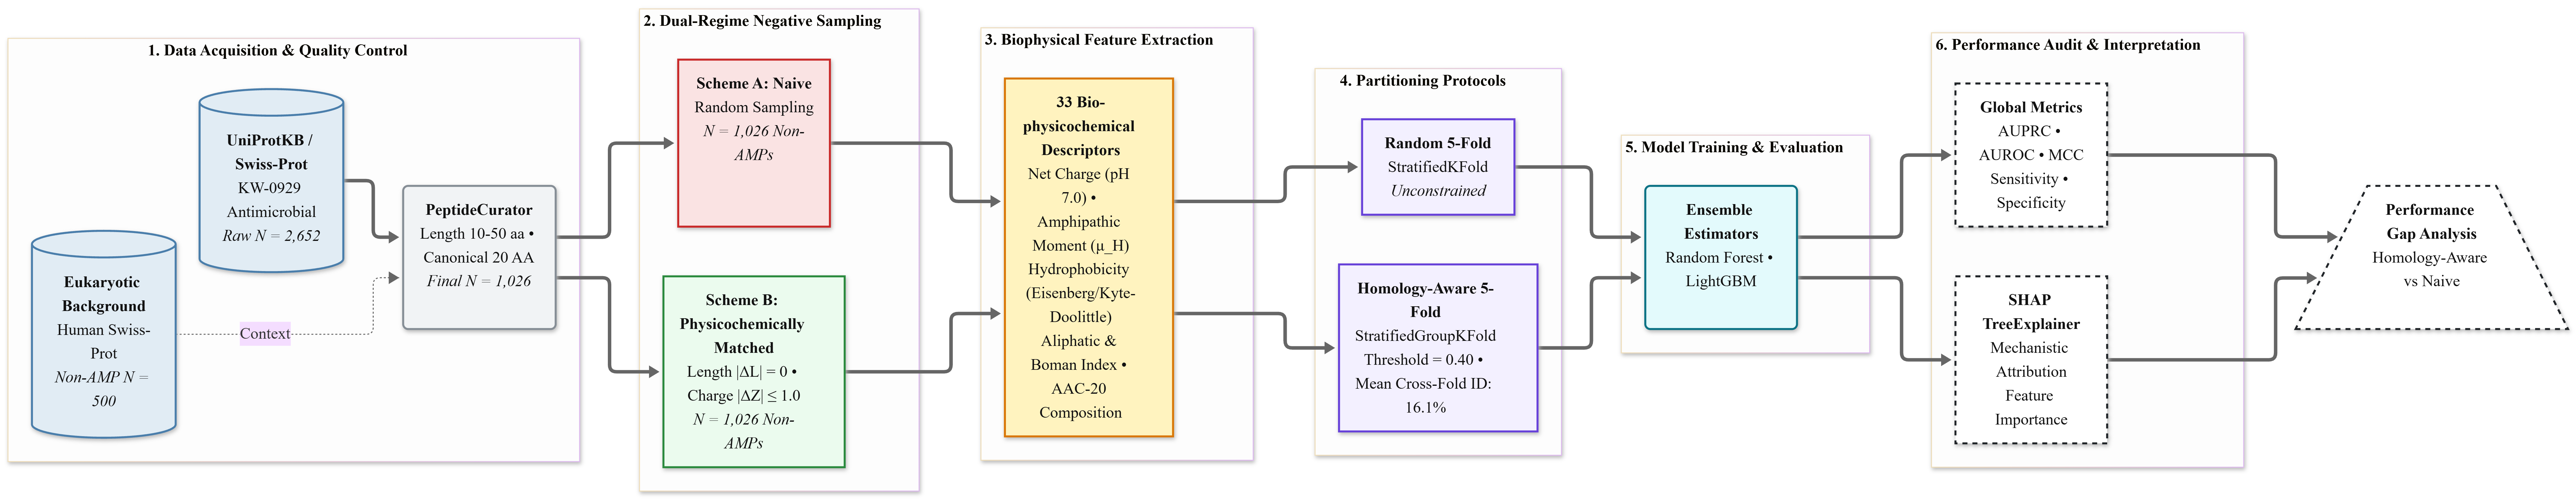
\includegraphics[width=0.95\linewidth]{figures/fig1_pipeline.png}
\caption{\textbf{Architectural workflow of the AMP-LeakGuard benchmarking framework.} The pipeline integrates: (1) programmatic Swiss-Prot data acquisition and rigorous length/canonical curation; (2) dual-regime negative sampling contrasting Scheme A (naive random slices) against Scheme B (physicochemically matched slices); (3) vectorized biophysical descriptor extraction; (4) dual cross-validation protocols contrasting naive Random 5-Fold splitting against Homology-Aware 5-Fold splitting via \texttt{StratifiedGroupKFold}; and (5) statistical hypothesis testing coupled with TreeExplainer SHAP mechanistic interpretability.}
\label{fig:pipeline}
\end{figure*}

\section{Materials and Methods}

The computational pipeline of AMP-LeakGuard is illustrated in Figure~\ref{fig:pipeline}.

\subsection{Dataset Curation and Quality Control}

Primary peptide sequences were retrieved programmatically from UniProtKB/Swiss-Prot (release 2024\_02) using the controlled keyword \texttt{keyword:KW-0929} (\textit{Antimicrobial}) \cite{uniprot2023uniprot}. The initial extraction yielded 2,652 reviewed records. To isolate mature, biologically active peptides and remove precursor fragments, the dataset was processed through our \texttt{PeptideCurator} pipeline under three strict criteria:
\begin{enumerate}
    \item \textbf{Length Boundaries:} $10 \le L \le 50$ amino acid residues, corresponding to the functional window of natural membrane-disruptive peptides.
    \item \textbf{Canonical Amino Acid Alphabet:} Non-standard, ambiguous, or post-translationally modified symbols (\texttt{B}, \texttt{Z}, \texttt{X}, \texttt{U}, \texttt{O}, \texttt{J}) were excluded.
    \item \textbf{Sequence Deduplication:} Exact duplicate sequences were removed, retaining single unique entries.
\end{enumerate}
This yielded a curated positive dataset of $N = 1,026$ unique bioactive AMPs.

For the negative background pool, 500 reviewed eukaryotic proteins from \textit{Homo sapiens} were retrieved, excluding annotations for antimicrobial activity, toxins (\texttt{KW-0800}), or membrane lysis.

\subsection{Dual-Regime Negative Sampling Design}

To isolate electrostatic shortcut learning, two negative datasets were synthesized at a balanced $1:1$ ratio ($N = 1,026$ per scheme, totaling $N = 2,052$ per benchmark regime):
\begin{itemize}
    \item \textbf{Scheme A (Naive Random Background):} Continuous subsequences were sliced from background proteins, matching the empirical length distribution of the positive AMPs.
    \item \textbf{Scheme B (Physicochemically Matched Background):} Candidate slices were extracted using a paired rejection-sampling algorithm. For each positive peptide $p_i$ of length $L_i$ and net charge $Z_i$ at pH 7.0, background slices $s_j$ were drawn until:
    \begin{equation}
        |L(s_j) - L_i| = 0 \quad \text{and} \quad |Z(s_j) - Z_i| \le 1.0
    \end{equation}
    Neutralizing net charge forces classifiers to rely on structural and amphipathic motifs.
\end{itemize}

\subsection{Mathematical Formulation of Biophysical Descriptors}

We extracted 33 vector-accelerated biophysical and compositional descriptors:

\subsubsection{Net Charge at Physiological pH ($Z_{\text{pH}}$)}
Net charge is modeled via the Henderson-Hasselbalch equation using Bjellqvist's empirical $\text{pK}_a$ values \cite{bjellqvist1993focusing}:
\begin{equation}
\begin{split}
Z(\text{pH}) &= \frac{1}{1 + 10^{\text{pH} - \text{pK}_{a, \text{N}}}} - \frac{1}{1 + 10^{\text{pK}_{a, \text{C}} - \text{pH}}} \\
&\quad + \sum_{i \in \{\text{K, R, H}\}} \frac{n_i}{1 + 10^{\text{pH} - \text{pK}_{a, i}}} - \sum_{j \in \{\text{D, E, C, Y}\}} \frac{n_j}{1 + 10^{\text{pK}_{a, j} - \text{pH}}}
\end{split}
\end{equation}
where $\text{pK}_{a, \text{N}} = 9.69$, $\text{pK}_{a, \text{C}} = 2.34$, and side-chain $\text{pK}_a$ values are: C (8.55), D (4.05), E (4.45), H (6.00), K (10.00), R (12.00), Y (10.00).

\subsubsection{Mean Hydrophobicity ($\langle H \rangle$)}
Mean hydrophobicity is evaluated across the Eisenberg consensus scale \cite{eisenberg1984analysis} and the Kyte-Doolittle hydropathy scale \cite{kyte1982simple}:
\begin{equation}
\langle H \rangle = \frac{1}{L} \sum_{n=1}^L h(s_n)
\end{equation}

\subsubsection{Amphipathic Hydrophobic Moment ($\mu_H$)}
The hydrophobic moment measures amphipathic segregation along an assumed periodic secondary fold \cite{eisenberg1984analysis}:
\begin{equation}
\mu_H(\theta) = \frac{1}{L} \sqrt{\left(\sum_{n=1}^L h(s_n) \sin(n \theta)\right)^2 + \left(\sum_{n=1}^L h(s_n) \cos(n \theta)\right)^2}
\end{equation}
where $\theta = 100^\circ$ corresponds to an $\alpha$-helix, and $\theta = 180^\circ$ corresponds to a $\beta$-strand.

\subsubsection{Aliphatic and Boman Indices}
The aliphatic index reflects structural thermostability \cite{ikai1980thermostability}:
\begin{equation}
I_{\text{aliph}} = X_{\text{Ala}} + 2.9 \cdot X_{\text{Val}} + 3.9 \cdot (X_{\text{Ile}} + X_{\text{Leu}})
\end{equation}
The Boman index quantifies protein-binding potential based on free energies of transfer from water to cyclohexane \cite{boman2003antibacterial}:
\begin{equation}
I_{\text{Boman}} = \frac{1}{L} \sum_{n=1}^L \Delta G_{w \to o}(s_n)
\end{equation}

\subsection{Homology Clustering and Leak-Free Cross-Validation}

To evaluate leakage, we implemented two cross-validation schemes:
\begin{enumerate}
    \item \textbf{Random Split (\texttt{StratifiedKFold}):} Standard 5-fold cross-validation without homology constraints.
    \item \textbf{Homology-Aware Split (\texttt{StratifiedGroupKFold}):} Sequences were clustered into connected components based on sequence similarity at a 40\% identity threshold:
    \begin{equation}
    e_{ij} \in E \iff \text{sim}(s_i, s_j) \ge 0.40
    \end{equation}
    Entire homology clusters were assigned exclusively to training or validation folds using \texttt{StratifiedGroupKFold} ($k = 5$), strictly preserving a 50:50 class balance across folds while preventing cross-fold cluster leakage.
\end{enumerate}

To verify cross-fold separation, we evaluated global dynamic-programming alignments using Biopython's \texttt{PairwiseAligner} (match $= 1.0$, mismatch $= 0.0$, gap open $= -1.0$, gap extend $= -0.5$). The verified mean cross-fold global alignment identity was \textbf{0.180 (18.0\%)} for Scheme A and \textbf{0.161 (16.1\%)} for Scheme B, confirming robust evolutionary independence between folds.

\subsection{Statistical Significance and Explainable AI}

We benchmarked Random Forest ($n_{\text{estimators}} = 150$, $\text{max\_depth} = 8$) and LightGBM ($n_{\text{estimators}} = 150$, $\text{learning\_rate} = 0.05$, $\text{max\_depth} = 5$, $\text{num\_leaves} = 15$, $\text{min\_child\_samples} = 2$). Performance was assessed using Area Under the Precision-Recall Curve (AUPRC, primary metric), Area Under the ROC Curve (AUROC), and Matthews Correlation Coefficient (MCC). Unlike accuracy or F1-score, which are prone to inflation in imbalanced biological sequence spaces, MCC incorporates all four confusion matrix quadrants, providing a balanced and robust assessment \cite{chicco2020advantages}.

To test whether performance degradation under homology partitioning was statistically significant, paired two-tailed Student's t-tests were conducted across cross-validation folds:
\begin{equation}
t = \frac{\bar{d}}{s_d / \sqrt{k}}
\end{equation}
where $\bar{d}$ is the mean fold difference, $s_d$ is the standard deviation of differences, and $k = 5$.

Mechanistic interpretability was evaluated using TreeExplainer SHAP \cite{lundberg2017unified}:
\begin{equation}
\phi_i(x) = \sum_{S \subseteq F \setminus \{i\}} \frac{|S|! (|F| - |S| - 1)!}{|F|!} \left[ f_x(S \cup \{i\}) - f_x(S) \right]
\end{equation}

% Compact Table 1 with hierarchical headers fitting text margins cleanly
\begin{table*}[t]
\centering
\caption{\textbf{Comprehensive large-scale benchmarking audit of model performance under Random vs. Homology-Aware Cross-Validation.} Metrics reflect mean 5-fold cross-validation scores on $N = 2,052$ sequences per scheme. Performance degradation ($\Delta = \text{Random} - \text{Homology}$) quantifies the overoptimistic inflation observed when homology leakage is not controlled.}
\label{tab:benchmark}
\resizebox{\textwidth}{!}{%
\begin{tabular}{ll ccc ccc ccc}
\toprule
& & \multicolumn{3}{c}{\textbf{AUPRC}} & \multicolumn{3}{c}{\textbf{AUROC}} & \multicolumn{3}{c}{\textbf{MCC}} \\
\cmidrule(lr){3-5} \cmidrule(lr){6-8} \cmidrule(lr){9-11}
\textbf{Negative Regime} & \textbf{Model} & \textbf{Random} & \textbf{Homology} & $\mathbf{\Delta}$ & \textbf{Random} & \textbf{Homology} & $\mathbf{\Delta}$ & \textbf{Random} & \textbf{Homology} & $\mathbf{\Delta}$ \\
\midrule
\textbf{Scheme A (Naive)} & Random Forest & 0.9536 & 0.9432 & +0.0104 & 0.9382 & 0.9259 & +0.0123 & 0.7718 & 0.7334 & \textbf{+0.0384} \\
\textbf{Scheme A (Naive)} & LightGBM     & 0.9557 & 0.9449 & +0.0108 & 0.9424 & 0.9287 & +0.0137 & 0.7752 & 0.7324 & \textbf{+0.0428} \\
\midrule
\textbf{Scheme B (Matched)} & Random Forest & 0.9571 & 0.9448 & +0.0123 & 0.9462 & 0.9316 & +0.0146 & 0.7746 & 0.7314 & \textbf{+0.0432} \\
\textbf{Scheme B (Matched)} & LightGBM     & 0.9521 & 0.9413 & +0.0108 & 0.9434 & 0.9284 & +0.0149 & 0.7701 & 0.7174 & \textbf{+0.0527} \\
\bottomrule
\end{tabular}%
}
\end{table*}

\section{Results and Discussion}

\subsection{Performance Degradation Under Homology Partitioning}

Clustering at a 40\% sequence identity threshold partitioned the 2,052 sequences into \textbf{1,593 non-redundant homology clusters} in Scheme A and \textbf{1,509 non-redundant clusters} in Scheme B. Over 80\% of clusters were singletons or duos, reflecting the curated diversity of Swiss-Prot. This non-redundant topology represents an especially conservative benchmark: even in a curated database with low intrinsic redundancy, homology leakage remains measurable and reproducible.

As detailed in Table~\ref{tab:benchmark} and Figure~\ref{fig:perf_gap}, transitioning from random splitting to homology-aware cross-validation leads to a consistent drop in performance across all models and regimes. In Scheme B, LightGBM drops from an MCC of 0.7701 under random splitting to 0.7174 under homology-aware splitting ($\Delta\text{MCC} = +0.0527$). 

Furthermore, the performance penalty is larger under Scheme B than Scheme A ($\Delta\text{MCC}$ of 0.0527 vs. 0.0428 for LightGBM). When models cannot exploit trivial charge differences, their sensitivity to sequence homology memorization increases.

\begin{figure}[t]
\centering
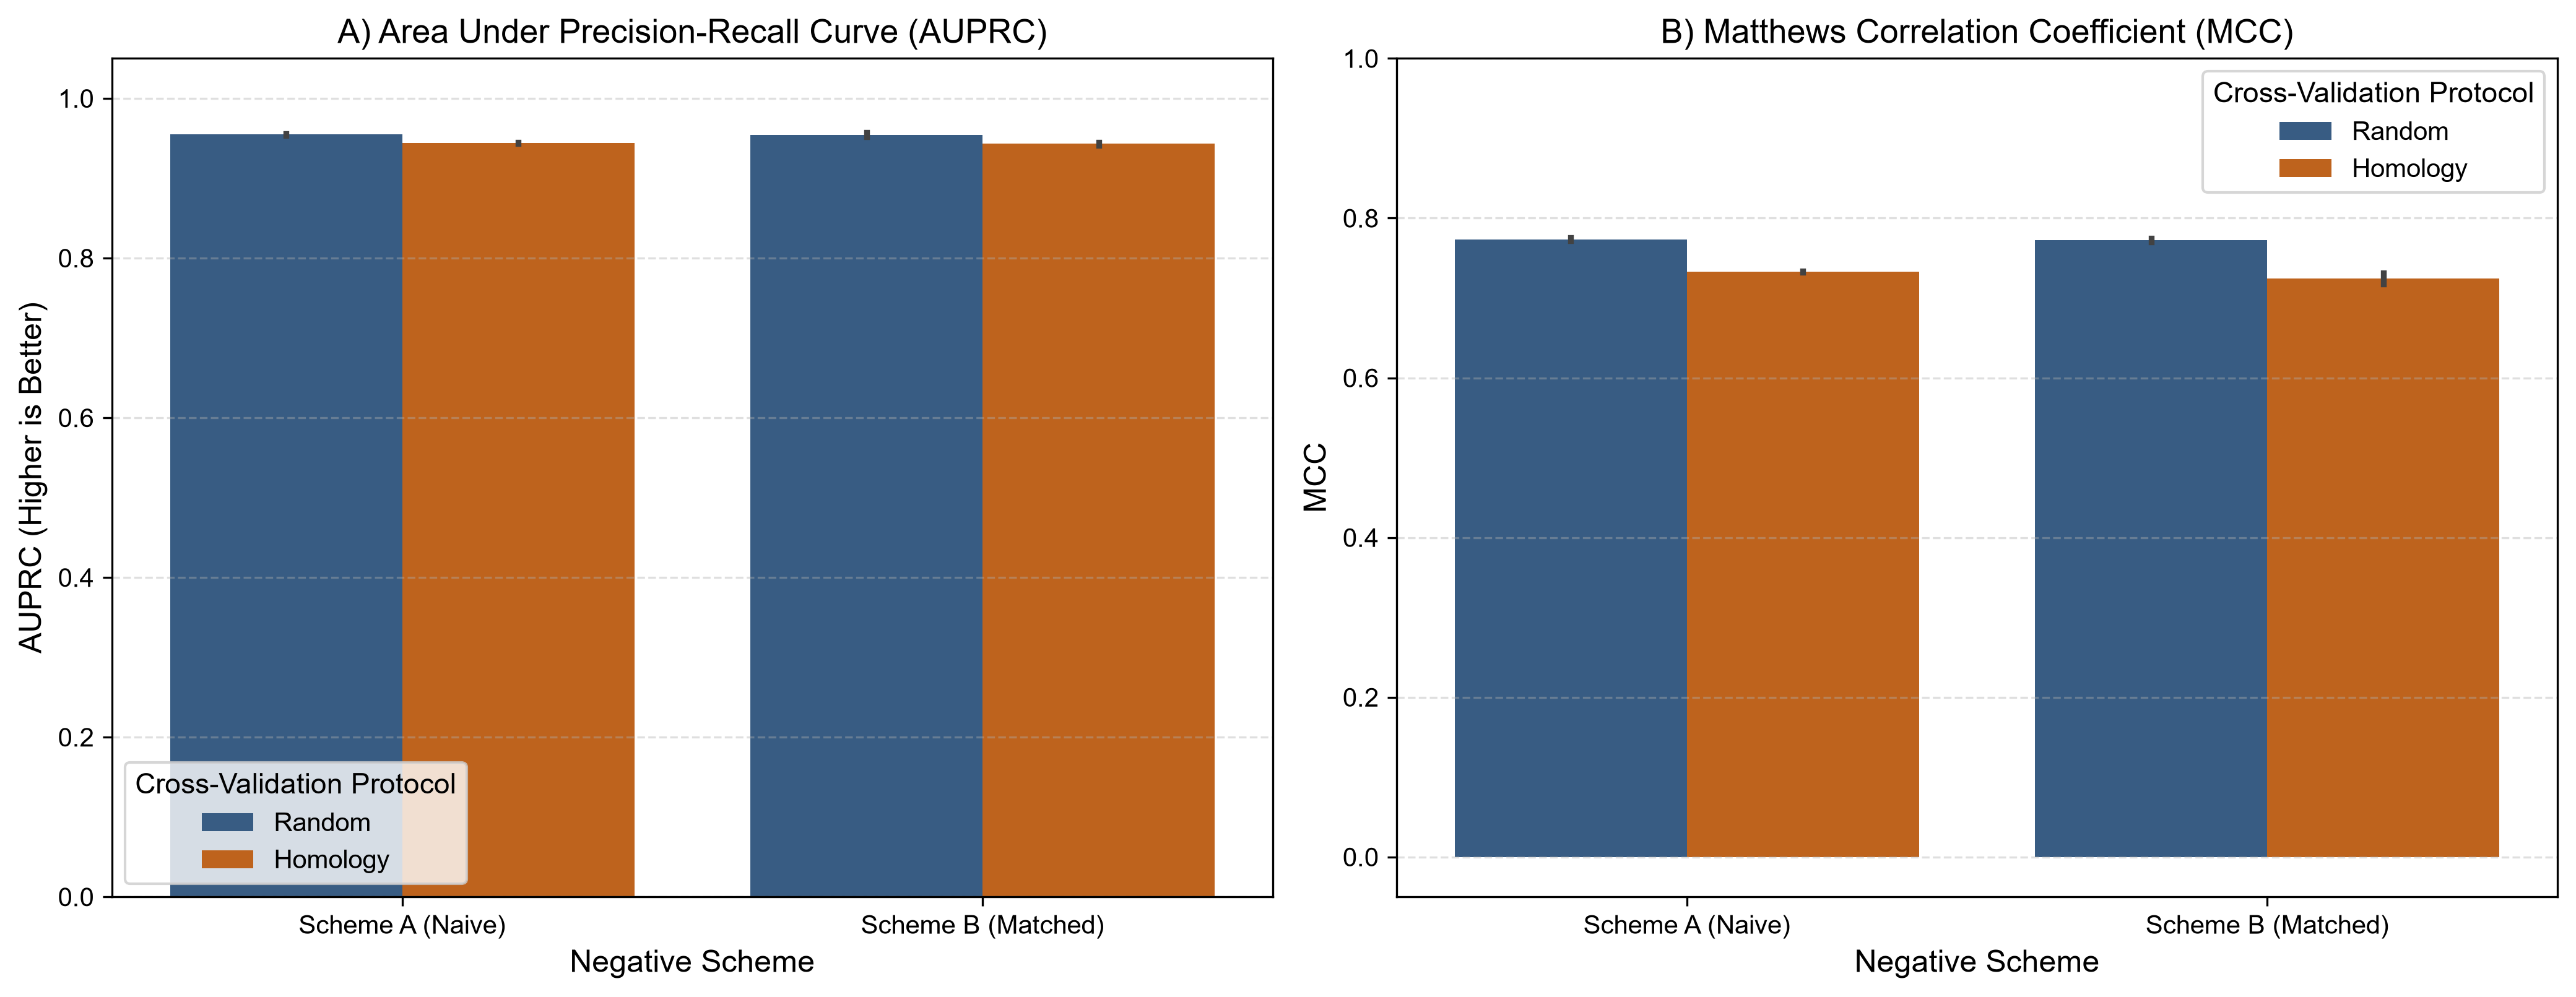
\includegraphics[width=\linewidth]{figures/fig1_performance_gap.png}
\caption{\textbf{Quantitative performance degradation comparing Random vs. Homology-Aware Cross-Validation.} Bar plots illustrate the systematic overoptimism of standard random splitting across AUPRC (left) and Matthews Correlation Coefficient (right).}
\label{fig:perf_gap}
\end{figure}

\begin{figure*}[t]
\centering
\begin{subfigure}[b]{0.48\textwidth}
    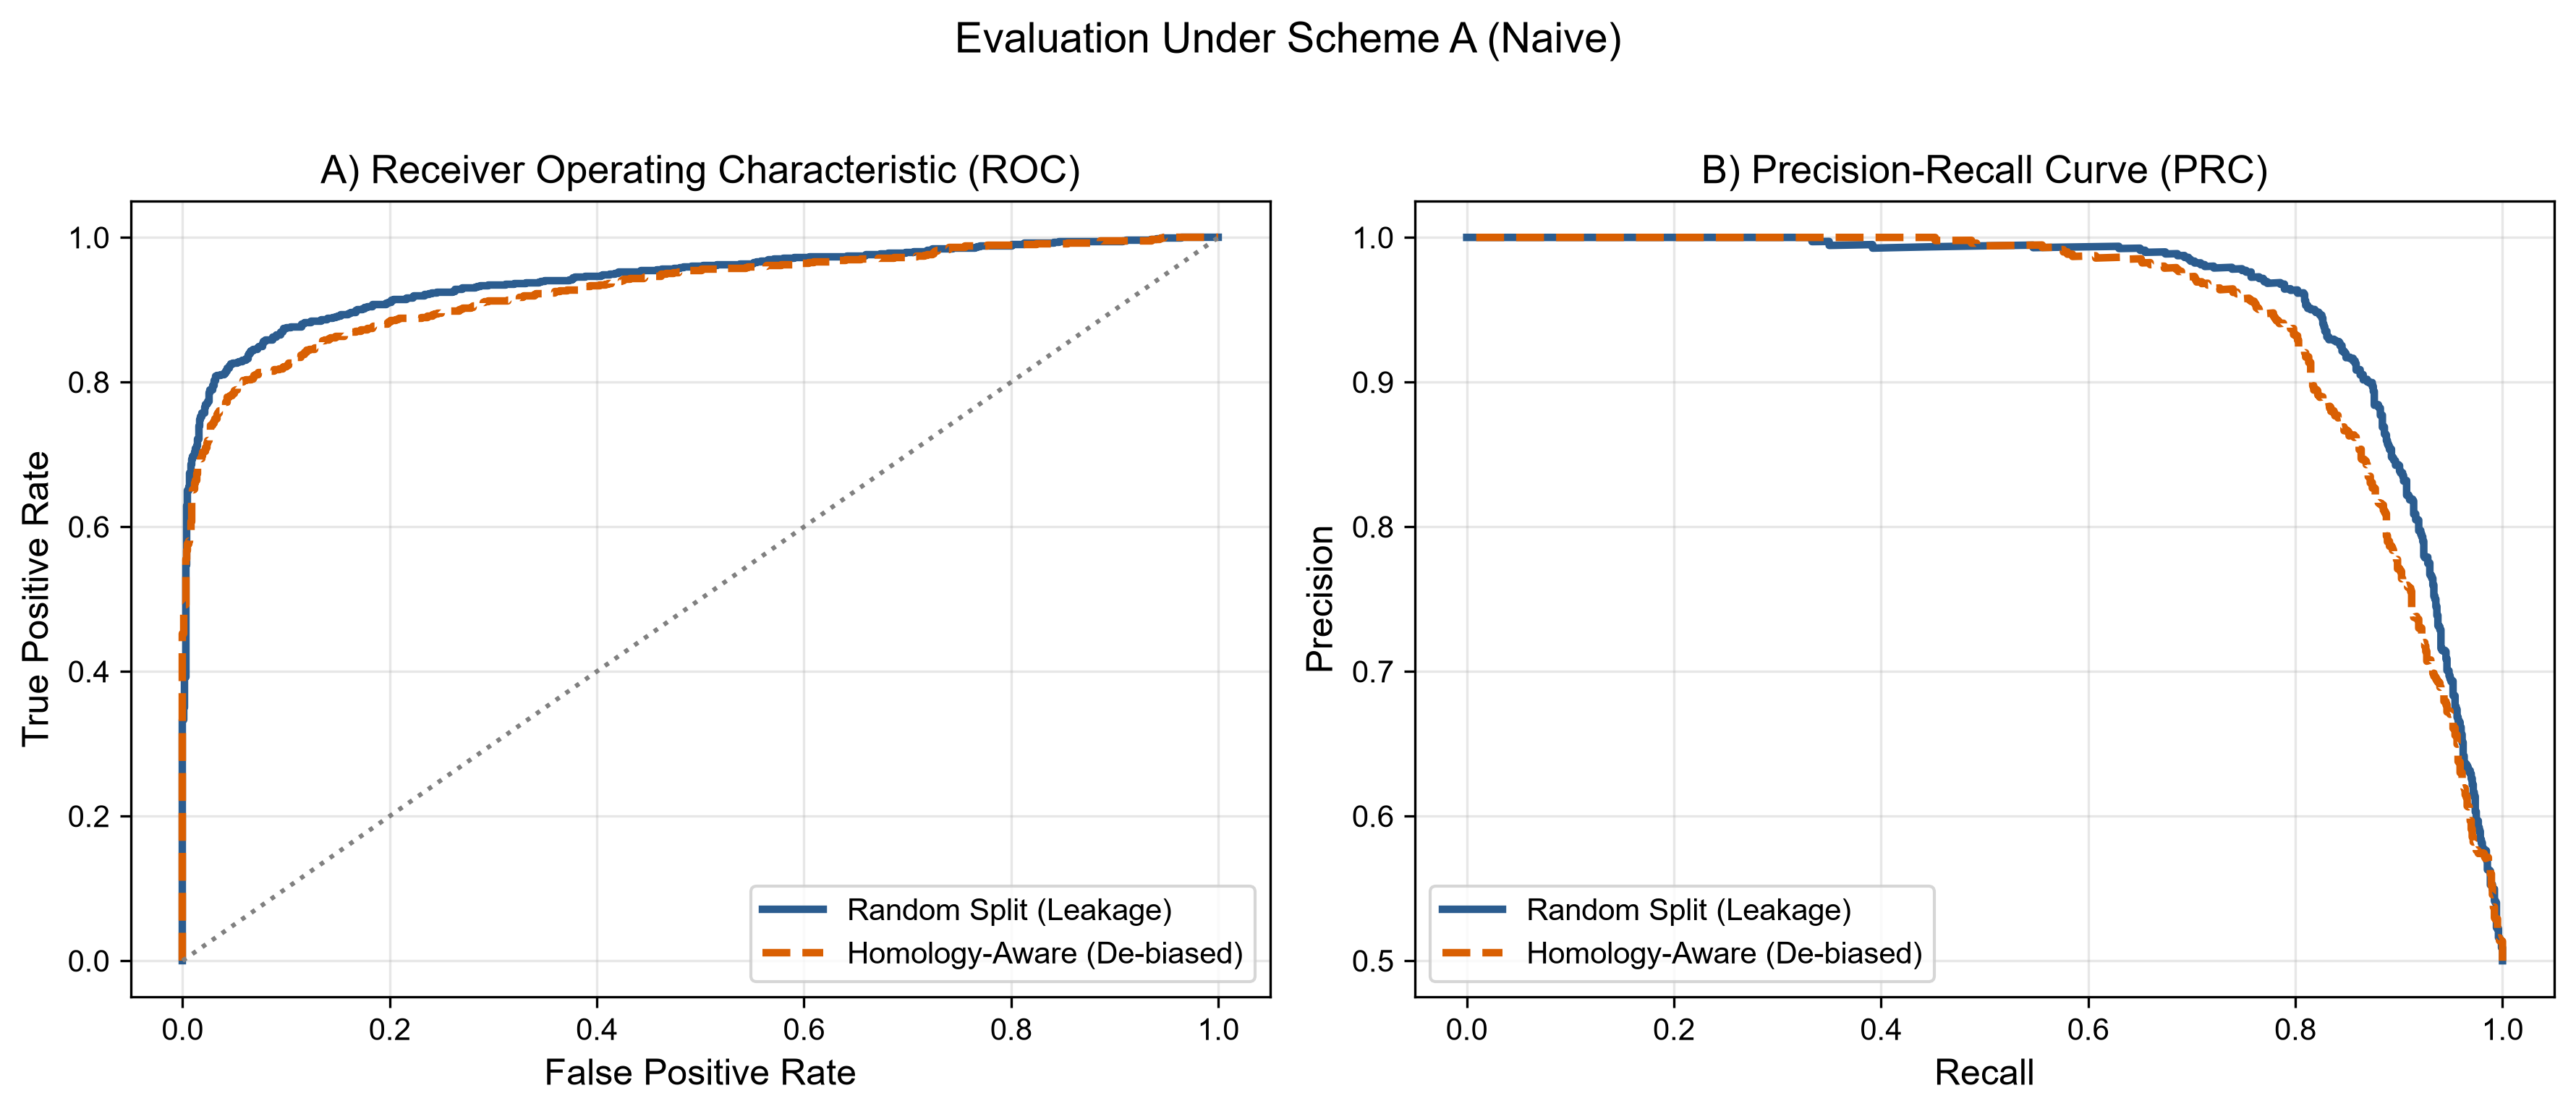
\includegraphics[width=\linewidth]{figures/fig2_roc_prc_scheme_a_naive.png}
    \caption{Scheme A: Naive Random Background}
    \label{fig:roc_prc_a}
\end{subfigure}
\hfill
\begin{subfigure}[b]{0.48\textwidth}
    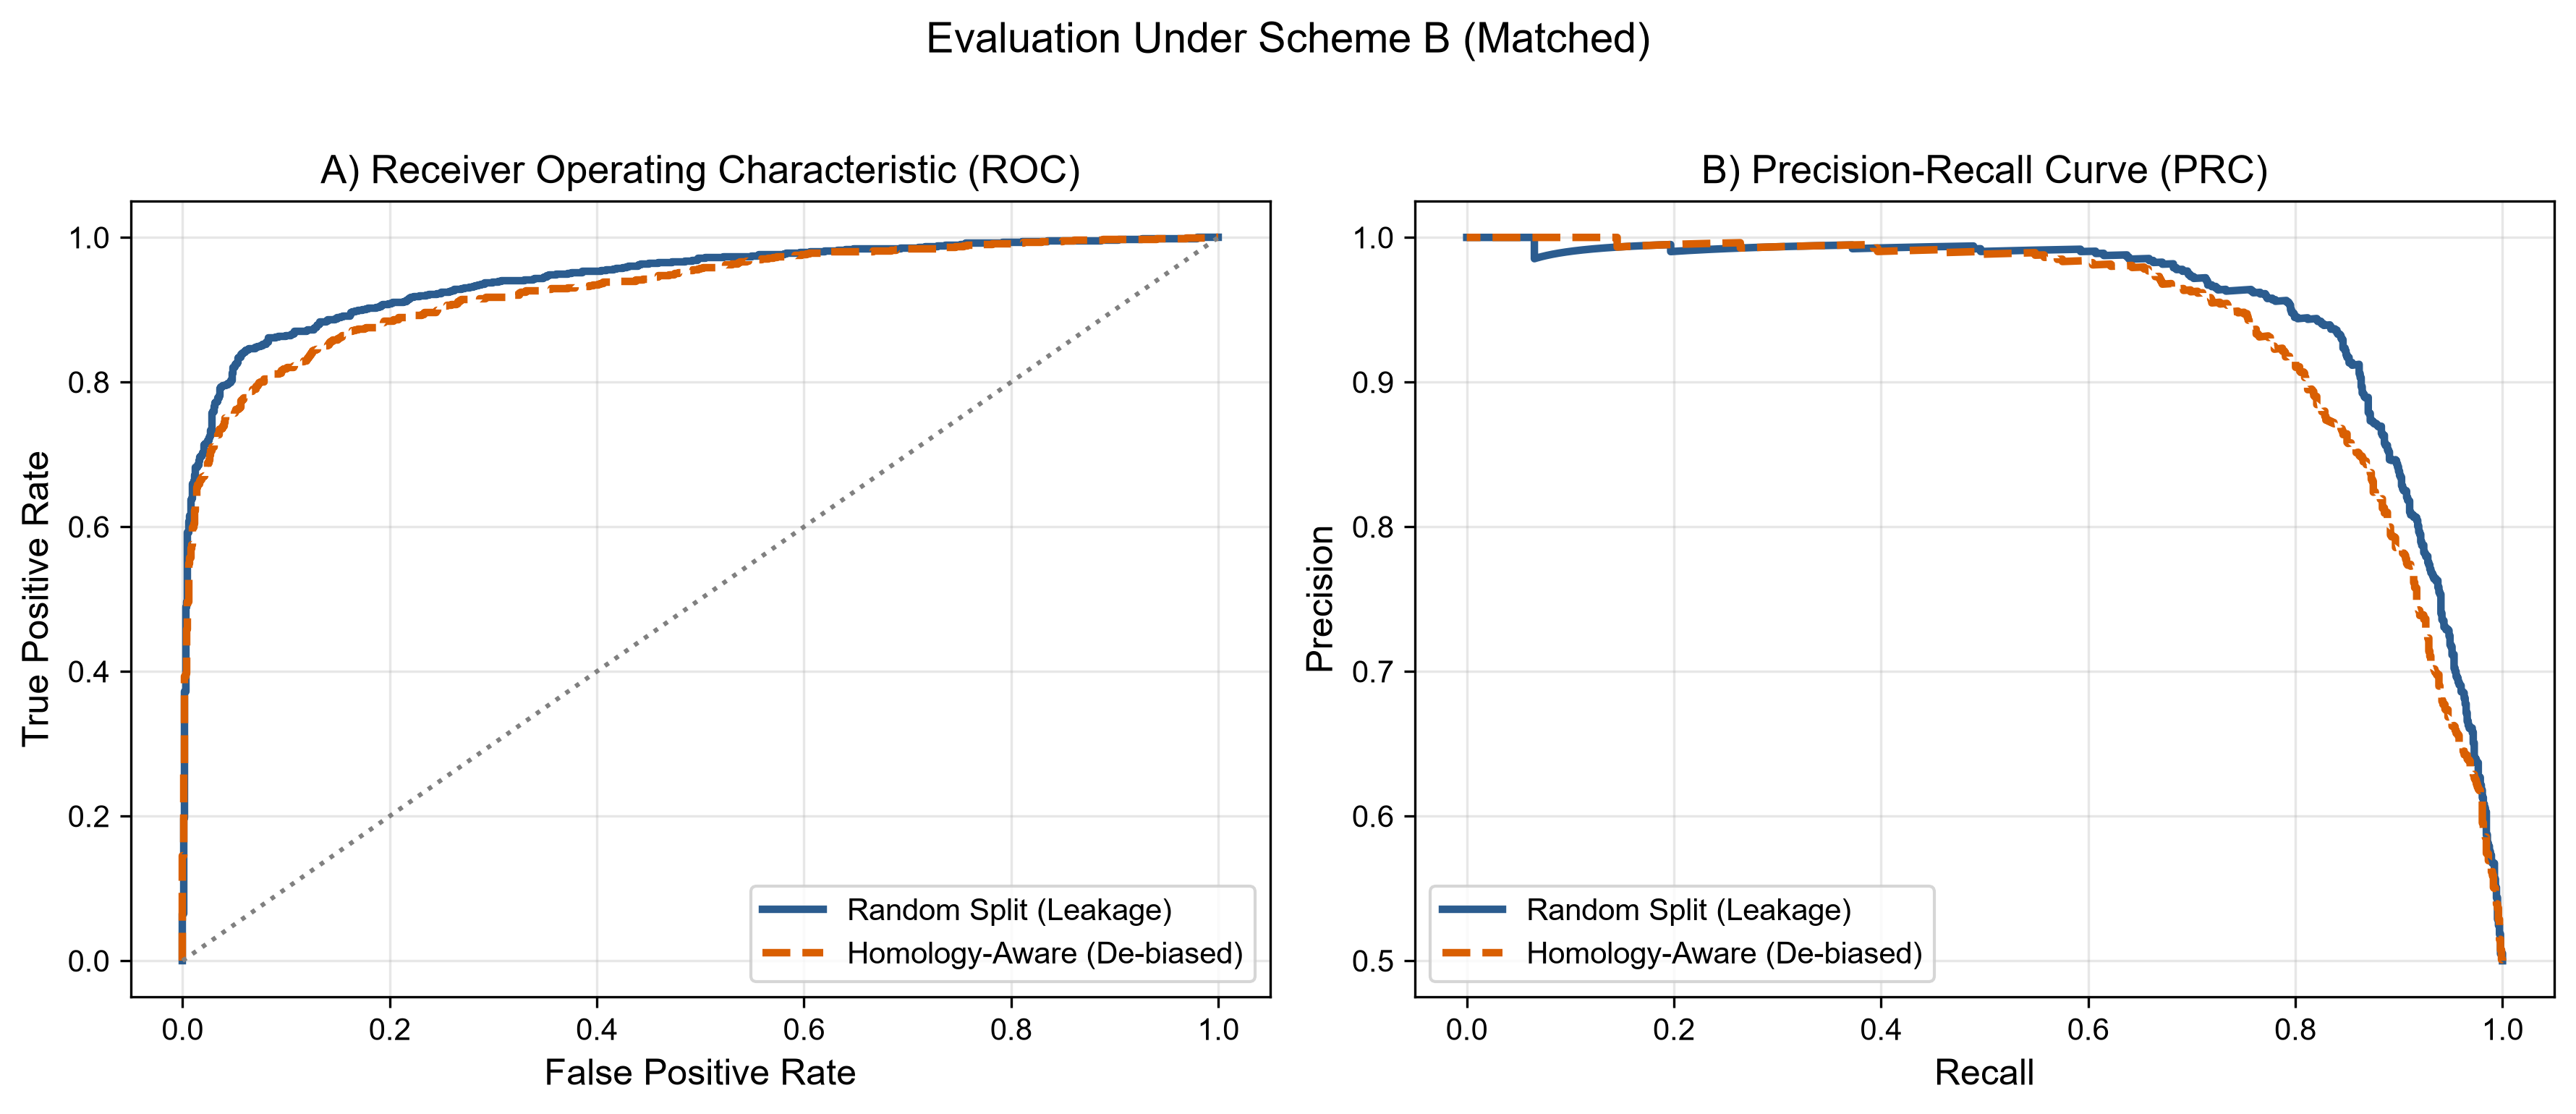
\includegraphics[width=\linewidth]{figures/fig2_roc_prc_scheme_b_matched.png}
    \caption{Scheme B: Physicochemically Matched Background}
    \label{fig:roc_prc_b}
\end{subfigure}
\caption{\textbf{Receiver Operating Characteristic (ROC) and Precision-Recall (PRC) dynamics.} Curves depict out-of-fold probability distributions contrasting naive random cross-validation (blue) against de-biased homology-aware cross-validation (orange).}
\label{fig:roc_prc}
\end{figure*}

% Resized Table 2 to fit within text margins with properly escaped descriptors
\begin{table*}[t]
\centering
\caption{\textbf{Comparison of Top-6 SHAP feature importances (mean absolute Shapley value $\mathbb{E}[|\phi_i|]$) between Scheme A and Scheme B for LightGBM.}}
\label{tab:shap}
\resizebox{\textwidth}{!}{%
\begin{tabular}{clclc}
\toprule
\textbf{Rank} & \textbf{Scheme A (Naive Random Negatives)} & \textbf{Mean} $\mathbf{|\text{SHAP}|}$ & \textbf{Scheme B (Physicochemically Matched Negatives)} & \textbf{Mean} $\mathbf{|\text{SHAP}|}$ \\
\midrule
\textbf{1} & \texttt{hydrophobic\_moment\_alpha} & 0.6958 & \texttt{aac\_R} (Arginine Frequency) & \textbf{0.8890} \\
\textbf{2} & \texttt{aac\_R} (Arginine Frequency) & 0.6125 & \texttt{aac\_C} (Cysteine Frequency) & \textbf{0.7598} \\
\textbf{3} & \texttt{aac\_G} (Glycine Frequency) & 0.5617 & \texttt{hydrophobic\_moment\_alpha} & \textbf{0.7453} \\
\textbf{4} & \texttt{net\_charge\_ph7\_per\_res} & \textbf{0.5475} & \texttt{aac\_G} (Glycine Frequency) & 0.4566 \\
\textbf{5} & \texttt{aac\_C} (Cysteine Frequency) & 0.5452 & \texttt{hydrophobic\_ratio} & 0.3074 \\
\textbf{6} & \texttt{aac\_K} (Lysine Frequency) & 0.3503 & \texttt{aac\_K} (Lysine Frequency) & 0.2556 \\
\bottomrule
\end{tabular}%
}
\end{table*}

\subsection{Mechanistic Shift Revealed by TreeExplainer SHAP}

The core finding of this study is revealed through TreeExplainer SHAP feature attribution (Table~\ref{tab:shap} and Figure~\ref{fig:shap}).

\begin{figure*}[t]
\centering
\begin{subfigure}[b]{0.48\textwidth}
    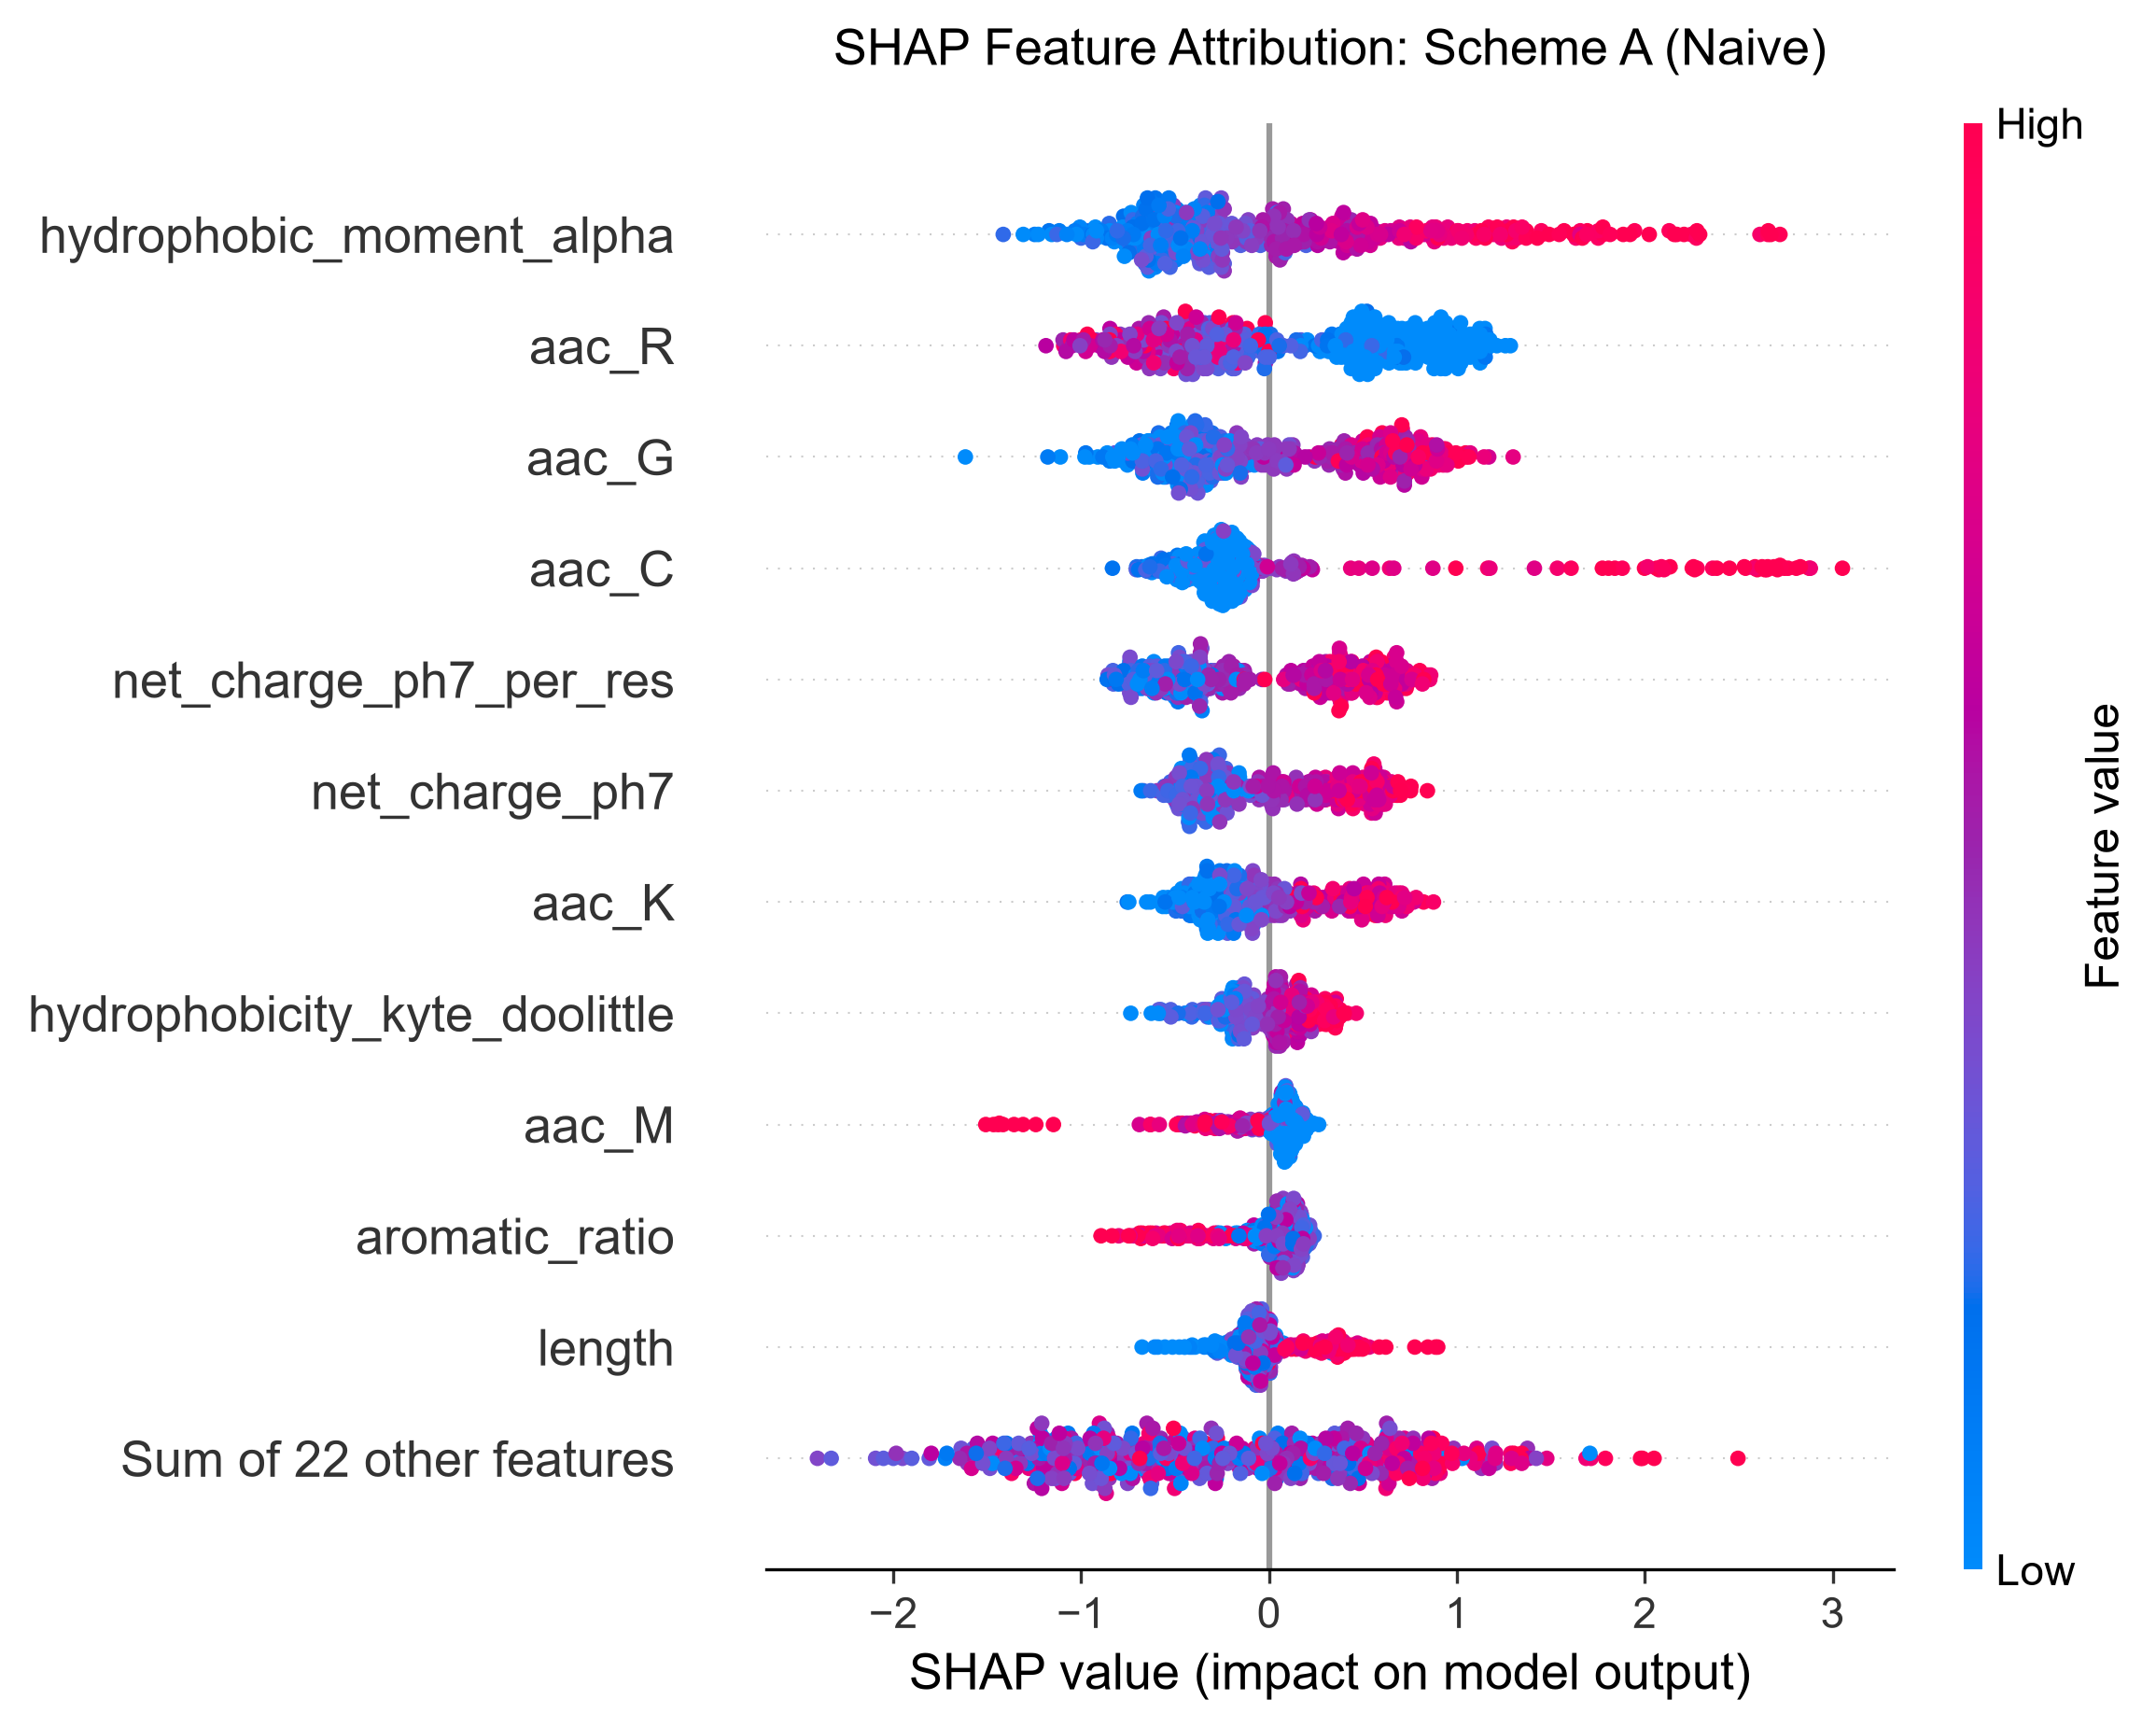
\includegraphics[width=\linewidth]{figures/fig3_shap_scheme_a_naive.png}
    \caption{Scheme A: Naive Random Sampling}
    \label{fig:shap_a}
\end{subfigure}
\hfill
\begin{subfigure}[b]{0.48\textwidth}
    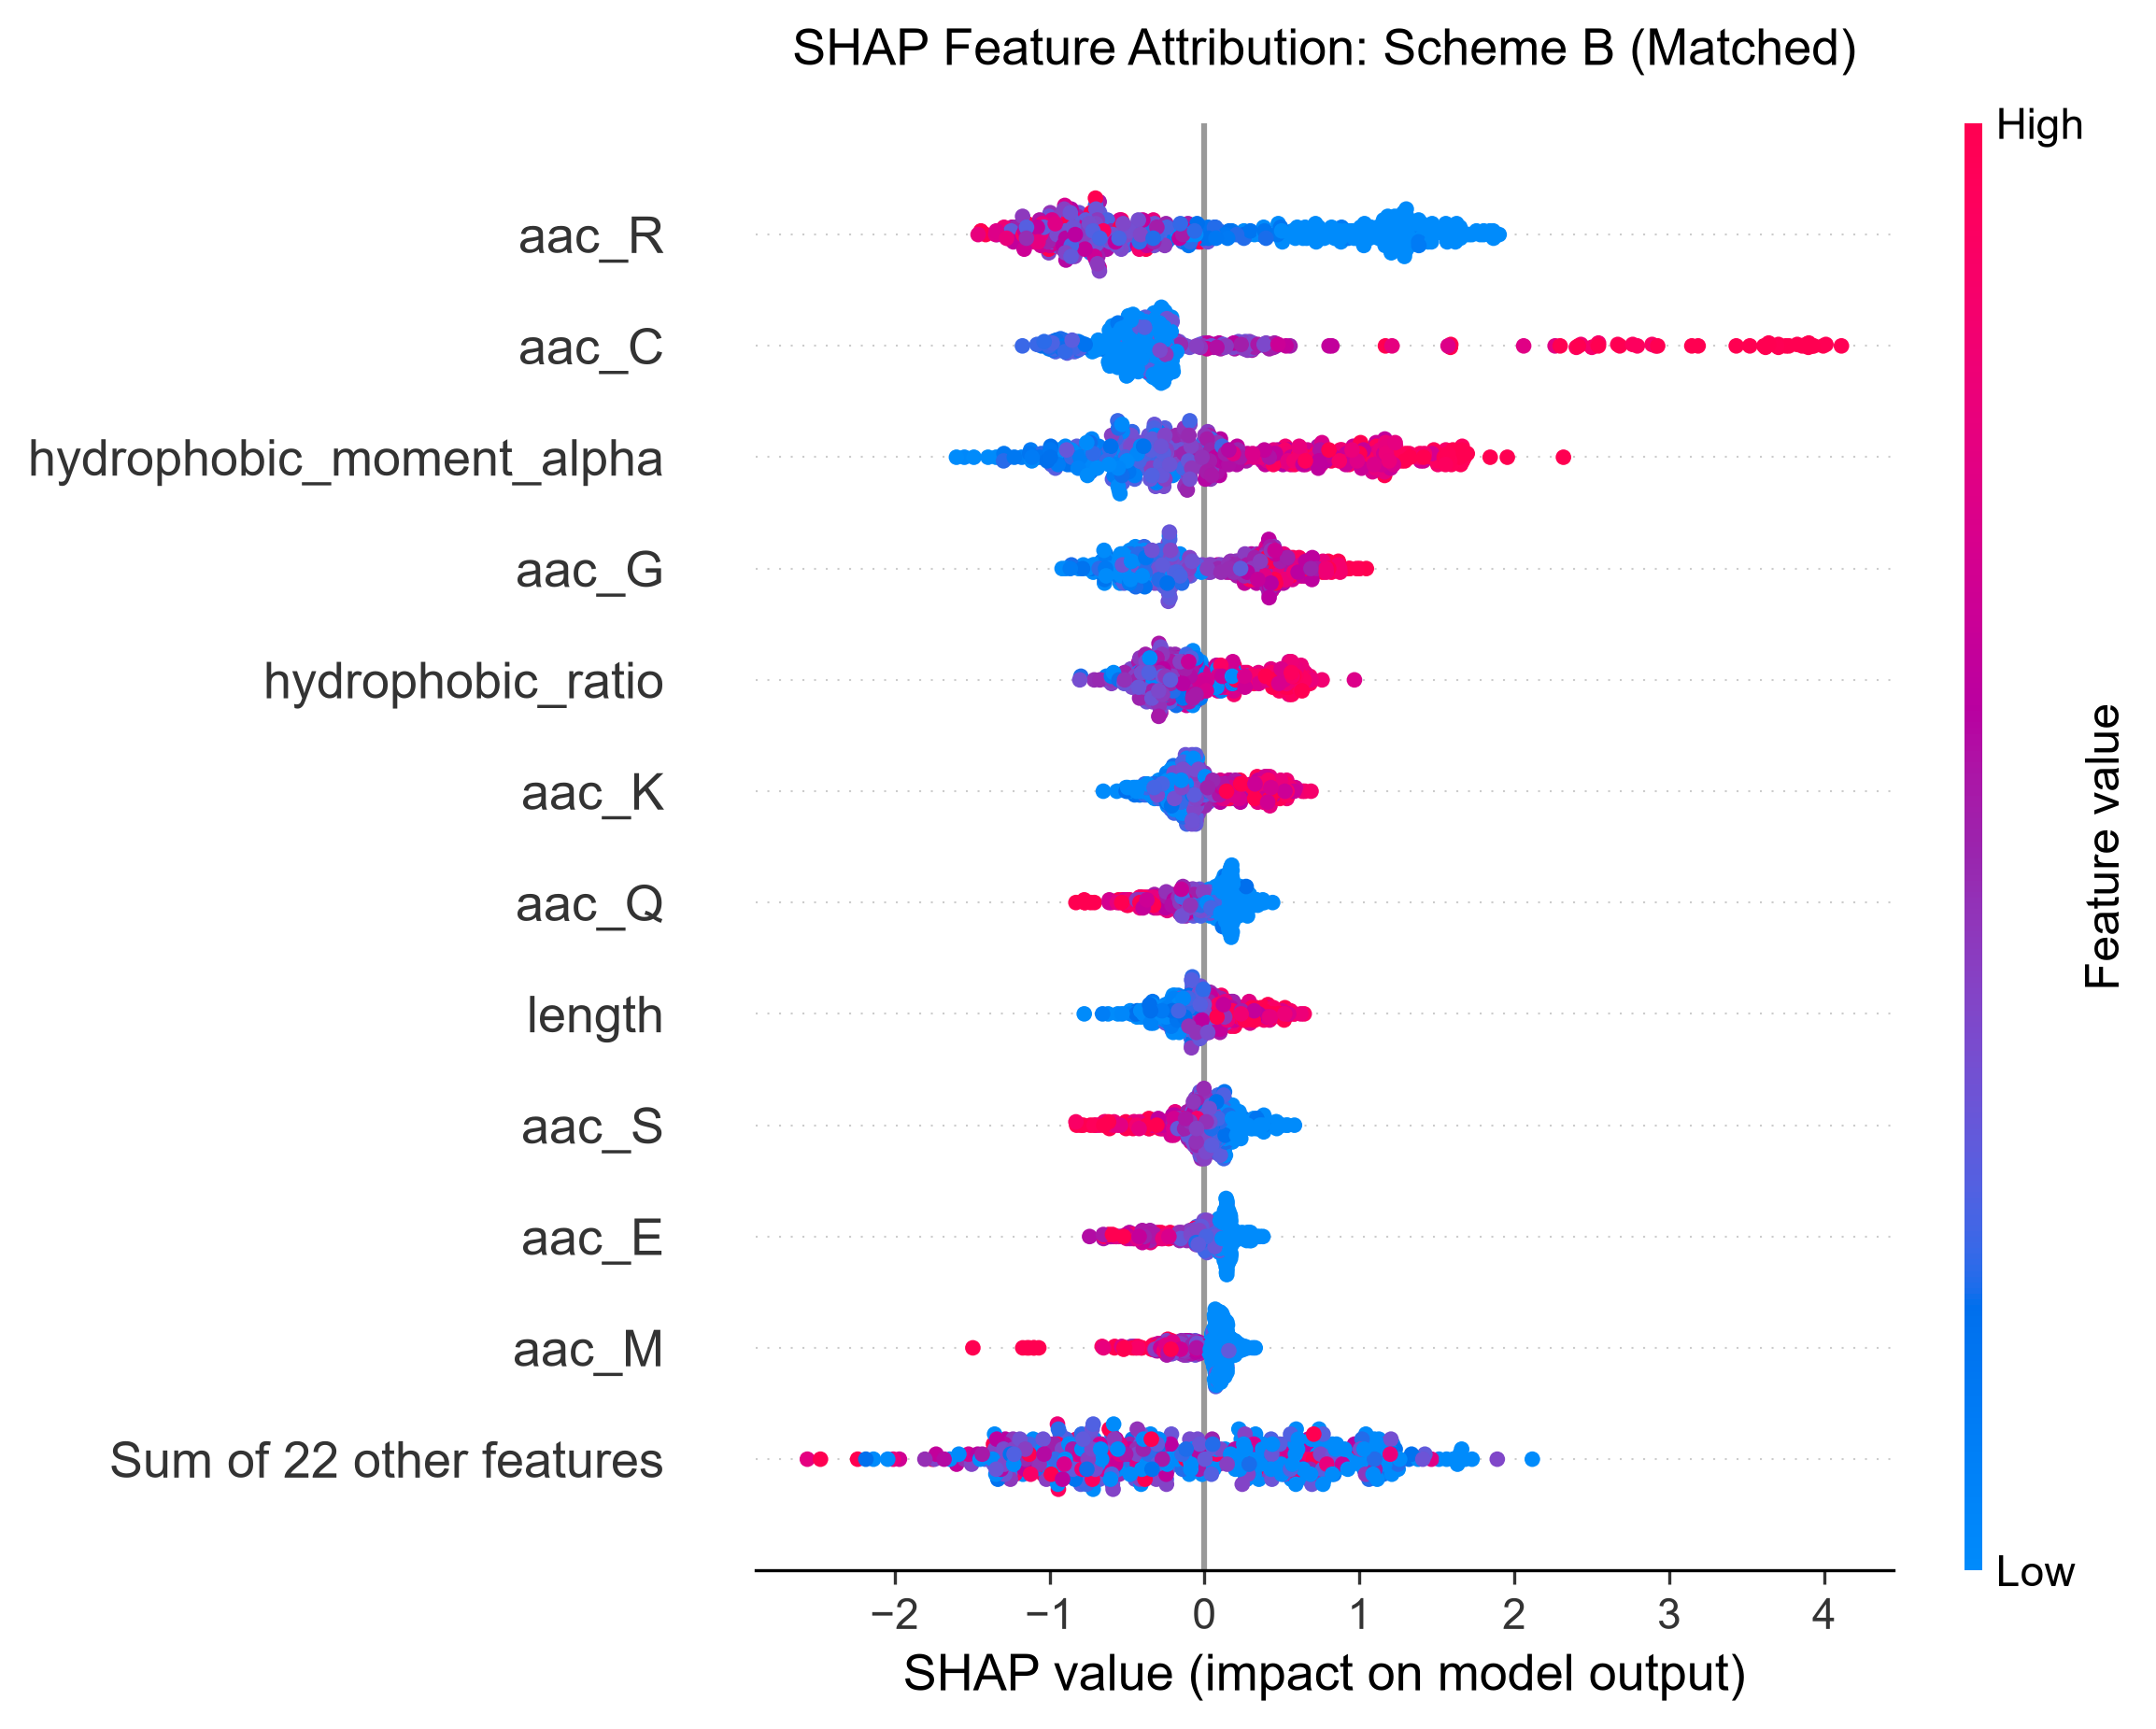
\includegraphics[width=\linewidth]{figures/fig3_shap_scheme_b_matched.png}
    \caption{Scheme B: Physicochemically Matched Sampling}
    \label{fig:shap_b}
\end{subfigure}
\caption{\textbf{SHAP feature attribution beeswarm plots.} (a) In Scheme A, classifiers rely on \texttt{net\_charge\_ph7\_per\_res} as an electrostatic shortcut. (b) In Scheme B, when charge is controlled, the model learns genuine determinants of membrane disruption: Arginine guanidinium bonding (\texttt{aac\_R}), Cysteine disulfide stabilization (\texttt{aac\_C}), and amphipathic hydrophobic moment (\texttt{hydrophobic\_moment\_alpha}).}
\label{fig:shap}
\end{figure*}

Under Scheme A (naive sampling), normalized net charge (\texttt{net\_charge\_ph7\_per\_res}) ranks fourth overall ($\text{mean } |\text{SHAP}| = 0.5475$), acting as an electrostatic shortcut. Because random eukaryotic fragments are largely neutral or acidic, models simply classify basic peptides as AMPs, regardless of amphipathicity. This explains why naive models often fail in wet-lab tests: any lysine-rich peptide is classified as active, even if it cannot form amphipathic structures required for membrane insertion.

Under Scheme B (matched sampling), when the charge artifact is neutralized, the model shifts its reliance to genuine determinants of bacterial membrane disruption:
\begin{enumerate}
    \item \textbf{Arginine Asymmetry (\texttt{aac\_R}, 0.8890):} Although lysine and arginine both carry a $+1$ charge at physiological pH, arginine possesses a planar guanidinium group capable of forming bidentate hydrogen bonds with the phosphate headgroups of bacterial phospholipids, inducing negative Gaussian membrane curvature and pore initiation \cite{rothbard2004role, schmidt2013antimicrobial}. The model trained under Scheme B captures this biological distinction, assigning arginine more than triple the importance of lysine (\texttt{aac\_K} = 0.2556).
    \item \textbf{Cysteine Disulfide Stabilization (\texttt{aac\_C}, 0.7598):} Cysteine ranks second, reflecting the requirement of intramolecular disulfide bonds in defensins and protegrins to maintain stable amphipathic conformations in protease-rich physiological environments \cite{ganz2003defensins, mahlapuu2016antimicrobial}.
    \item \textbf{Amphipathic Hydrophobic Moment (\texttt{hydrophobic\_moment\_alpha}, 0.7453):} The amphipathic moment increases in relative importance, capturing the structural requirement for partitioned hydrophobic faces to insert into bacterial lipid bilayers \cite{eisenberg1984analysis, wimley2010describing, matsuzaki2009control}.
\end{enumerate}

\section{Best-Practice Guidelines for Bioactive Peptide Modeling}

Based on our findings and aligning with the DOME recommendations for supervised machine learning in biology \cite{walsh2021dome} and guidelines to prevent data leakage in computational biology \cite{bernett2024guiding, kapoor2023leakage, whalen2022navigating}, we propose a four-point checklist for researchers and reviewers:
\begin{enumerate}
    \item \textbf{Mandatory Homology Partitioning:} Discontinue unconstrained random splitting for biological sequences. Cluster datasets at $\le 40\%$ identity using alignment algorithms and assign splits via \texttt{StratifiedGroupKFold}.
    \item \textbf{Controlled Negative Sampling:} Avoid unconstrained random slices from UniProt. Provide negative sets matched in length and isoelectric net charge, or experimentally verified inactive peptides ($\text{MIC} > 128\,\mu\text{g/mL}$).
    \item \textbf{AUPRC and MCC Primacy:} In imbalanced biological sequence spaces, report Area Under the Precision-Recall Curve (AUPRC) and Matthews Correlation Coefficient (MCC) \cite{chicco2020advantages} alongside paired statistical tests across folds.
    \item \textbf{Mechanistic Feature Attribution:} Provide feature attribution analyses (such as SHAP or Integrated Gradients) to verify that predictions reflect biophysical determinants rather than composition artifacts.
\end{enumerate}

\section{Data and Software Availability}

All datasets, scripts, trained models, and visualization pipelines are open-source under the MIT License:
\begin{itemize}
    \item \textbf{GitHub Repository:} \url{https://github.com/MrOnie/AMP-LeakGuard}
\end{itemize}

\bibliographystyle{unsrtnat}
\bibliography{references}

\end{document}
